
\documentclass{beamer}


\usetheme{Warsaw}
\usecolortheme{crane}


\title{Tensor Analysis}
\subtitle{Mathematical Methods in the Physical Sciences}
\author{Steve Mazza}
\institute[Naval Postgraduate School]
{ 
    Naval Postgraduate School \\
    Monterey, CA \\
    
\includegraphics[height=3cm]{images/NPS_logo.jpg}
}
\date {SE3030, Winter/2014 \\ Quantitative Methods of Systems Engineering}
\subject{Quantitative Methods of Systems Engineering}


\begin{document}

\frame{\titlepage}


\frame{{Introduction}
  \begin{columns}[c]
  \column{.6\textwidth}
  \begin{itemize}
    \item Tensors are designated by their size and \emph{order}.
    \item Tensors of order 0 are scalars
    \item Tensors of order 1 are vectors
    \item A second order tensor has $3^2=9$ components
  \end{itemize}
  \column{.5\textwidth}
    \begin{center}
      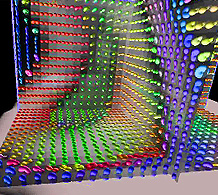
\includegraphics[scale=0.6]{images/tensors.jpg}
    \end{center}
  \end{columns}
}


\frame{{Cartesian Tensors}
  Under \emph{passive rotation} the vectors are fixed and the axes are rotated.  We want to know how the components of a displacement vector in one coordinate system are related to its components in a rotated system. A vector $\vec{r}$ has components $x, y, z$ or $x', y', z'$ relative to the two coordinate systems.
  \begin{table}
    \centering
    \begin{tabular}{c|ccc}
      &$x$&$y$&$z$ \\
      \hline
      $x'$&$l_1$&$m_1$&$n_1$ \\
      $y'$&$l_2$&$m_2$&$n_2$ \\
      $z'$&$l_3$&$m_3$&$n_3$ \\
    \end{tabular}
  \end{table}
  The table lists the cosines of the nine angles between the $(x,y,z)$ and the $(x',y',z')$ axes.
}


\frame{{Cartesian Tensors (continued)}
  Let $\vec{i}, \vec{j}, \vec{k}$ be unit vectors along $(x,y,z)$ axes and $\vec{i'}, \vec{j'}, \vec{k'}$ be unit vectors along $(x',y',z')$.  Then we can represent $\vec{r}$ as follows.
  \begin{align*}
    r &= \vec{i}x + \vec{j}y + \vec{k}z = \vec{i'}x' + \vec{j'}y' + \vec{k'}z' \\
    \vec{r}\cdot\vec{i} &= \vec{i}\cdot\vec{i'}x + \vec{j}\cdot\vec{i'}y + \vec{k}\cdot\vec{i'}z = x' \\
    \text{since } \vec{i'}\cdot\vec{i'} &= 1, \text{ and } \vec{i'}\cdot\vec{j'} = \vec{i'}\cdot\vec{k'} = 0 \\
    \text{and } \vec{i}\cdot\vec{i'} &= l_1, \vec{j}\cdot\vec{i'} = m_1, \vec{k}\cdot\vec{i'} = n_1 \\
    x' &= l_1x + m_1y + n_1z \\
    y' &= l_2x + m_2y + n_2z \\
    z' &= l_3x + m_3y + n_3z
  \end{align*}
  These are the transformation equations from $(x,y,z)$ to $(x', y', z')$.
}


\frame{{Tensor Notation and Operations}
  \begin{itemize}
    \item For simplicity, we drop the summation sign and assume summation over any index which appears twice in one term.
    \item Contraction
      \begin{itemize}
        \item Obtained by setting unlike indices equal and summing
        \item Reduces the order by 2
      \end{itemize}
    \item First and second order tensors can be displayed as matrices.
    \item Symmetry
      \begin{itemize}
        \item Symmetric if $T_{ij}=T_{ji}$.
        \item Antisymmetric if $T_{ij}=-T_{ji}$.
        \item Any second order tensor can be written as a sum of a symmetric and antisymmetric tensor.
      \end{itemize}
    \item Combination
      \begin{itemize}
        \item The linear combination of two tensors of order $n$ is a tensor of order $n$.
        \item Addition is not defined for tensors of different order.
      \end{itemize}
    \item Quotient Rule is useful for identifying components of a tensor.
  \end{itemize}
}


\frame{{Inertia Tensor}
  For a rigid body rotating about a fixed axis, we know that the velocity, $\omega$, and momentum, $L$, are related by the equation $L=I\omega$ where $I$ is the moment of inertia.  But if the rotation axis is not fixed, then $I$ must be replaced by a second order tensor with components $I_{jk}$.
}


\frame{{Kronecker Delta and Levi-Civita Symbol}
  \begin{block}{Kronecker Delta}
    \[
    \delta_{ij} =
    \begin{cases}
    1 \text{ if } i=j \\
    0 \text{ otherwise}
    \end{cases}
    \]
  \end{block}
  \begin{block}{Levi-Civita Symbol}
  \[
    \epsilon_{ijk} = 
    \begin{cases}
      1 & \text{ for an even permutation } \\
      -1 & \text{ for an odd permutation } \\
      0 & \text{ if any indices are repeated}
    \end{cases}
  \]
  \end{block}
}


\frame{{Vector Identities}
  \begin{block}{3-by-3 determinant}
  	\[\text{det } A=a_{1i}a_{2j}c_{3k}\epsilon_{ijk}\]
  \end{block}
  \begin{block}{Dot Product}
  	\[A\cdot B = A_iB_i\]
  \end{block}
  \begin{block}{Cross Product}
  	\[\left(A\times B\right)_i = \epsilon_{ijk}B_jC_k\]
  \end{block}
  \begin{block}{Curl}
  	\[\left(\nabla\times V\right)_i = \epsilon_{ijk}\frac{\partial}{\partial x_j}V_k\]
  \end{block}
}
	

\frame{{Pseudovectors and Pseudotensors}
  The general case of orthogonal transformations includes reflections.
  \begin{itemize}
    \item If $\text{det } A=1$ (rotation), it is called a \emph{polar} or true vector.
    \item If $\text{det } A=-1$ (reflection), it is called an \emph{axial} or pseudovector.
  \end{itemize}
}


\frame{{More About Applications}
  %TODO: Enter reminder. (mazzas) Tue Feb 18 07:33:53 2014
}


\frame{{Curvilinear Coordinates}
  %TODO: Enter reminder. (mazzas) Tue Feb 18 07:33:53 2014
}


\frame{{Vector Operations in Orthogonal Curvilinear Coordinates}
  %TODO: Enter reminder. (mazzas) Tue Feb 18 07:33:53 2014
}


\frame{{Non-Cartesian Tensors}
  %TODO: Enter reminder. (mazzas) Tue Feb 18 07:33:53 2014
}


\frame{{Miscellaneous Problems}
  %TODO: Enter reminder. (mazzas) Tue Feb 18 07:33:53 2014
}


\frame{{Questions?}
	\begin{center}
		
\includegraphics[width=.7\textwidth]{images/fin.png}
	\end{center}
}

\end{document}
